\begin{frame}[plain]% The optional argument 'plain' hides the headline and footline
	\begin{center}\bfseries\centering
		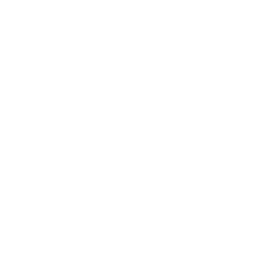
\includegraphics[scale=1]{Feathergraphics/cse_logo_opa0}
		%		\includegraphics[scale=1]{\; \;}
		\vspace{-5.75cm} \\
		{\adjustbox{scale=3}{\color{cseblue} II. Cotangent Space}}
		\bigskip\bigskip % Vertical whitespace
		{\ }\vspace{4cm}\\
		\bigskip
	\end{center}
\end{frame}

\begin{frame}[fragile]{\textbf{II. Cotangent Space}}{Vectors and Covectors}
\begin{center}\LARGE
``Vectors = columns''\quad and\quad ``Covectors = rows''	
\end{center}
\end{frame}
\begin{frame}[fragile]{\textbf{II. Cotangent Space}}{Vectors and Covectors}		
Fix any point $p\in S^1$.
\begin{itemize}
	\item[]
	\item[$\bullet$] A vector $\vec{v}\in T_pS^1$ is a column \[
	\vec{v}=\begin{bmatrix}
		v_1\\ v_2
	\end{bmatrix}
	\] satisfying $xv_1+yv_2=0$.
	\item[]
	\item[$\bullet$] A covector $\lambda$ is a linear functional on $T_pS^1$; represent it a a row \textbf{row} $\begin{bmatrix}
		\alpha & \beta
	\end{bmatrix}$ acting by \[
	\lambda(\vec{v})= \begin{bmatrix}
		\alpha & \beta
	\end{bmatrix}=\begin{bmatrix}
	v_1\\ v_2
\end{bmatrix}\alpha v_1+\beta v_2.
	\]
\end{itemize}
\end{frame}

\begin{frame}[fragile]{\textbf{II. Cotangent Space}}{Cotangent Space}
Define \[
T_p^*S^1:=\mathrm{Hom}(T_pS^1,\mathbb{R})=\set{\;\text{rows acting linearly on columns in $T_pS^1$}\;}.
\]
\ \\
\vspace{40pt}
\textbf{Note.}\; Columns live in $T_pS^1$, rows live in $T_p^*S^1$.
\end{frame}

\begin{frame}[fragile]{\textbf{II. Cotangent Space}}{1-form as a dual of vector field}
	Define \begin{align*}
		TS^1:=\bigsqcup_{p\in S^1}T_pS^1=\set{(p,\vec{v}):p\in S^1, \vec{v}\in T_pS^1}\\
		T^*S^1:=\bigsqcup_{p\in S^1}T_p^*S^1=\set{(p,\lambda):p\in S^1, \lambda\in T_pS^1}.
	\end{align*}\ \\
	\textbf{Note.}
	\begin{enumerate}[$\bullet$]
		\item[]
		\item  A \textbf{vector field} is a map $\vec{X}:S^1\to TS^1$.
		\item  A \textbf{1-form} is a map $\omega:S^1\to T^*S^1$.
	\end{enumerate}\vfill
For example, \[
\vec{F}(x,y)=\begin{bmatrix}
	-y \\ x
\end{bmatrix},\quad\quad \omega=(-y)dx+xdy.
\]
\end{frame}


\begin{frame}[fragile]{\textbf{II. Cotangent Space}}{Line integrals: vector vs. 1-form}
Let $\gamma:[a,b]\to S^1$.
\begin{enumerate}[$\bullet$]
	\item \textbf{Line Integral of Vector-field}: \[
	\int_{S^1}\vec{F}\cdot d\vec{r}=\int_{[a,b]}\vec{F}(\gamma(t))\cdot\gamma'(t)\; dt.
	\]
	\item \textbf{Line Integral of 1-form}: \[
	\int_{S^1}\omega=\int_{[a,b]}\omega_{\gamma(t)}(\gamma'(t))\; dt.
	\]
\end{enumerate}
\end{frame}
